%---------------------------------------------------------------------------
% Monitoring Hub component.
%
%---------------------------------------------------------------------------
\section{Monitoring Hub}
\label{sec:arch_monitoring_hub}

Monitoring Hub is the core component of the system. If using layered model to analyze application, Monitoring Hub should be treated as logic layer - placed between the presentation layer (GUI) and data access layer (transport proxies). It provides services to GUI and it uses Transport Proxy implementations and Knowledge component. Its main responsibilities include resources management (registering new resources, discovery dependent resources), measurements management (creation, pausing, resuming and termination) and creation of scheduled jobs that pools for capability values and pushes new values to registered listeners.

When user wants to start monitoring new resource, He or She must choose which Monitoring Hub to use. This decision, creates direct association between the chosen hub, the resource to monitor and all its child resources discovered during registration. This association defines that Monitoring Hub associated during registration and discovery process will process all further request calls related to given resource.

To make high-level components loosely coupled, Monitoring Hub is not aware of details about other components. To be able to provide its services it uses transport proxies and knowledge components, but it interacts with them only using commonly known interfaces. Additionally it is not aware about the existence of GUI component at all. It just provide services by implementing given interface, and it uses also common listener interfaces to notify about a variety of events.


\subsection{Decomposition of Monitoring Hub}

\begin{figure}[ht]
\centering
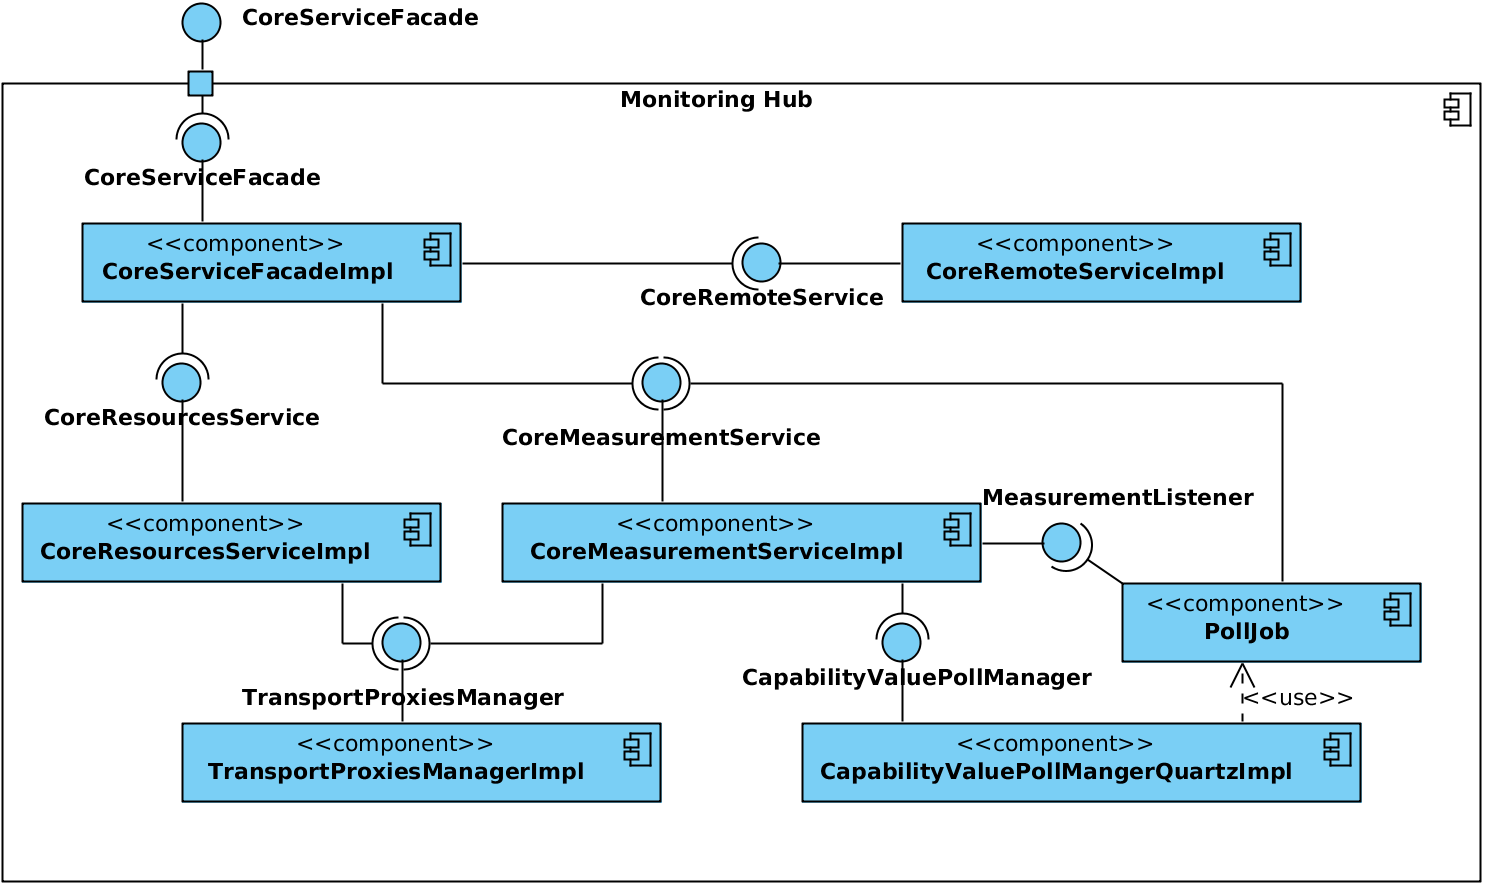
\includegraphics[width=0.9\textwidth]{decomposition_mon_hub}
\caption{Communication diagram - adding of new resource}
\label{fig:decomposition_mon_hub}
\end{figure}

Further decomposition of Monitoring Hub can be found in Figure~\ref{fig:decomposition_mon_hub}. This module is composed of following low level components:

\begin{itemize}

\item {\bf CoreServiceFacadeImpl}~~~~~~~~~~~~~~~~~~~~~~~~~~~~~~~~~~~~~~~~~~~~~~~~~~~~~~~~\linebreak
CoreServiceFacadeImpl is a facade that allows access to all Monitoring Hub functionalities from a single interface (CoreServiceFacade, shared with GUI and Monitoring Hub Application high level components). This wrapper eases remote access by exposing and using one interface with any remoting middle ware is easier than multiple ones. Having multiple interfaces in most cases would require multiple socket connections which can be a source of additional problems. We should tend to use as small amount connections as possible, because more connections system uses, than it becomes more and more prone to network configuration issues (e.g. firewalls). Additionally, using single facade improves code style, as with facade, only one interface has to be visible for all other components that are its clients.

\item {\bf CoreRemoteServiceImpl}~~~~~~~~~~~~~~~~~~~~~~~~~~~~~~~~~~~~~~~~~~~~~~~~~~~~~~~~\linebreak
CoreRemoteServiceImpl is a service responsible for processing requests related to remote management of Monitoring Hub. It has two main responsibilities: it allows registering remote listening interfaces and it dispatches local events (new resource, new capability value etc.) to remote listeners in aggregated manner. Distributed dispatch of events requires a bit different approach than a local one (local one, means dispatch inside of single JVM process). First of all, in most cases remote interface that will receive notifications with different signature, to allow handling exceptions related to networking. Additionally, to reduce the amount of remote calls and thus improve efficiency, CoreRemoteServiceImpl aggregates events into batches and notifies remote listeners using a generated package of them. Such an approach does not pollute measuring results, because each measurement value has associated gather timestamp (see~\ref{subsec:arch_comm_protocol}), initialized by component that grabs given value, at the exact moment, of measurement. Additionally, as events related to resources addition/removal don\rq{}t require such a strict time association, those events can be aggregated without any issues.

\item {\bf CoreResourcesServiceImpl}~~~~~~~~~~~~~~~~~~~~~~~~~~~~~~~~~~~~~~~~~~~~~~~~~~~~~~~~\linebreak
CoreResourcesServiceImpl is responsible for resources management: registering new ones, discovery of their children, returning all registered and discovered ones. It is also used to get more details about a resource, like capabilities that given resource may have.

\item {\bf CoreMeasurementServiceImpl}~~~~~~~~~~~~~~~~~~~~~~~~~~~~~~~~~~~~~~~~~~~~~~~~~~~~~~~~\linebreak
The CoreMeasurementServiceImpl can be used to create, pause, stop or terminate a measurement. Additionally it gathers current values of capabilities. It is used by the PollJob component for that purpose. It implements the MeasurementListener interface to be able to receive notifications about new capability values polled by the PollJob. 

\item {\bf TransportProxiesManagerImpl}~~~~~~~~~~~~~~~~~~~~~~~~~~~~~~~~~~~~~~~~~~~~~~~~~~~~~~~~\linebreak
The TransportProxiesManagerImpl component manages registered transport proxies. It is used by other components to get all transport proxies or to lookup a transport proxy that can be used to manage given resource.

\item {\bf CapabilityValuePollManagerImpl}~~~~~~~~~~~~~~~~~~~~~~~~~~~~~~~~~~~~~~~~~~~~~~~~~~~~~~~~\linebreak
CapabilityValuePollManagerImpl is responsible for scheduling polling jobs that are needed to run measurement.

\item {\bf PollJob}~~~~~~~~~~~~~~~~~~~~~~~~~~~~~~~~~~~~~~~~~~~~~~~~~~~~~~~~\linebreak
PollJob gets triggered with a configured interval. It simply polls for current capability value and push it to listeners specified during a creation stage.

\end{itemize}

\pagebreak

\subsection{Most important data flows}

This section contains a description of most salient data flows inside Monitoring Hub component. It covers actions of adding new resources, adding new measurements and dispatching new capability value notification.

Figure~\ref{fig:comm_mh_add_res} depicts communication diagram of adding new resources. In this scenario, external GUI component initiates action - registerResource request is the first step send by GUI to CoreServiceFacadeImpl. Facade simply delegates this call to CoreResourcesServiceImpl, which will perform actual registration. In the next step, CoreResourcesServiceImpl tries to find proxy capable to communicate with given resource by calling TransportProxiesManagerImpl. What should be noticed here, Transport Proxy is an external component to Monitoring Hub. After successfully obtaining transport proxy, CoreResourcesServiceImpl performs call to register given resource. If this registration succeeds, the CoreResourcesServiceImpl uses external Knowledge component, to get all types of child resources. Using this list, service requests TransportProxy to discover all children of the registered resource. After successful discovery, notification containing resources is being dispatched to all listeners. This can be done either directly, when given Monitoring Hub is embedded into GUI or remotely, using CoreRemoteServiceImpl.

\begin{figure}[ht]
\centering
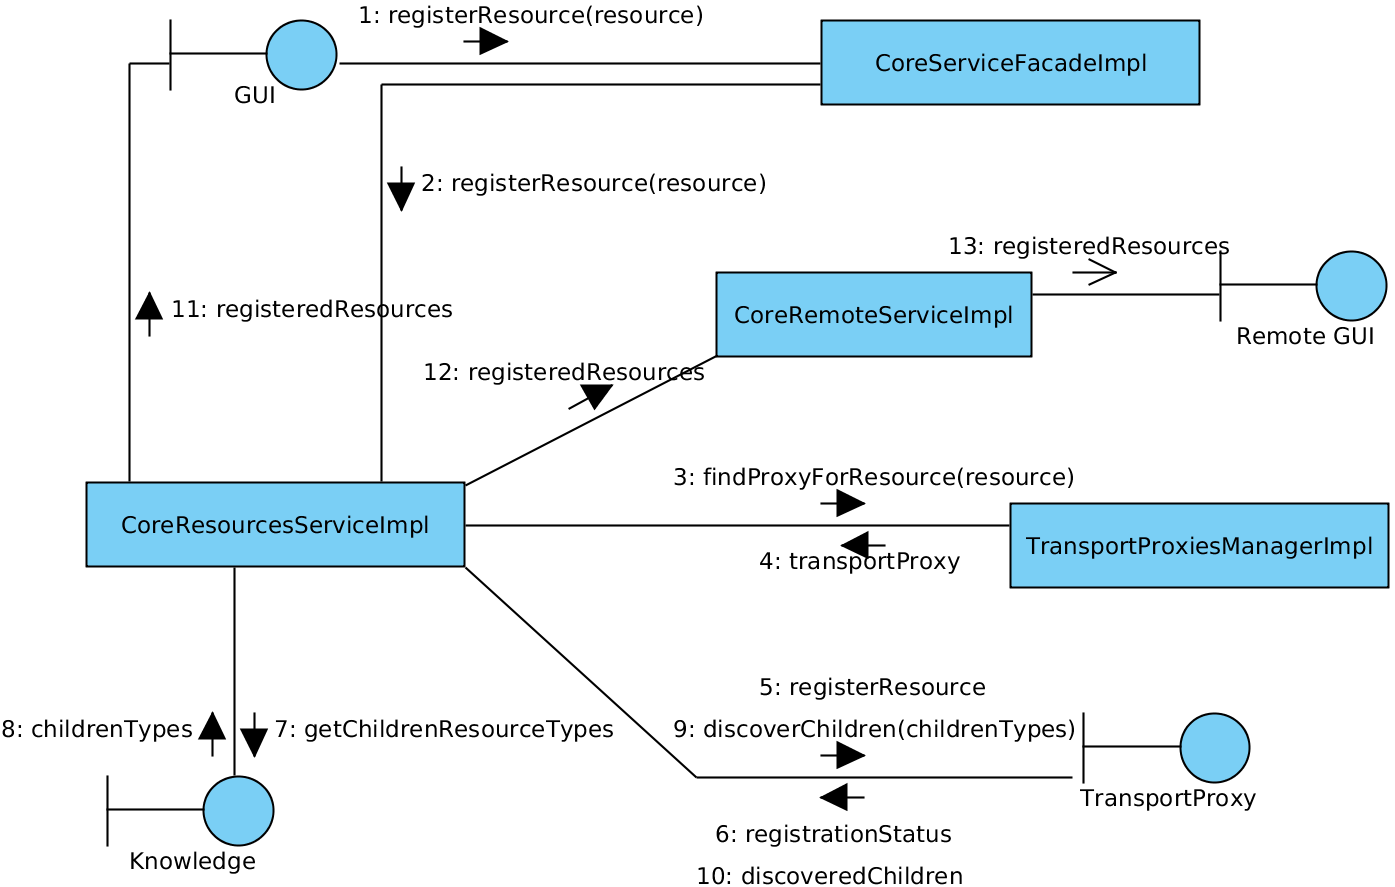
\includegraphics[width=0.9\textwidth]{comm_mh_add_res}
\caption{Monitoring Hub Communication diagram - adding new resource}
\label{fig:comm_mh_add_res}
\end{figure}

Communication diagram covering action of adding new measurements can be found in Figure~\ref{fig:comm_mh_add_measurement}. In this scenario, again GUI component is initiator. GUI component calls a getResourceCapabilities method, thus sends a first request to CoreServiceFacadeImpl. It will use those capabilities to show the user UI component, which will let user choose which capability should be measured. Facade delegates query to CoreResourcesServiceImpl, which passes it to external Knowledge component. Resulting list of capability URIs is being passed all way back, to the GUI component. Next, user selects, which capability should be measured. On selection event, GUI requests CoreServiceFacadeImpl to create measurement using given definition (see Table~\ref{tab:TO_MeasurementDef}). Request is delegated to CoreMeasurementServiceImpl which is responsible for the creation of measurement. Measurement service requests CapabilityValuePollManagerImpl to create a new instance of PollJob class. Measurement service, after creating polling job, generates measurement id, stores it internally with measurement definition, and returns it to requester. This identifier is then passed back to GUI, which will use it in any future call referring newly created measurement. Additionally it will be used to reference all incoming CapabilityValue objects.

\begin{figure}[ht]
\centering
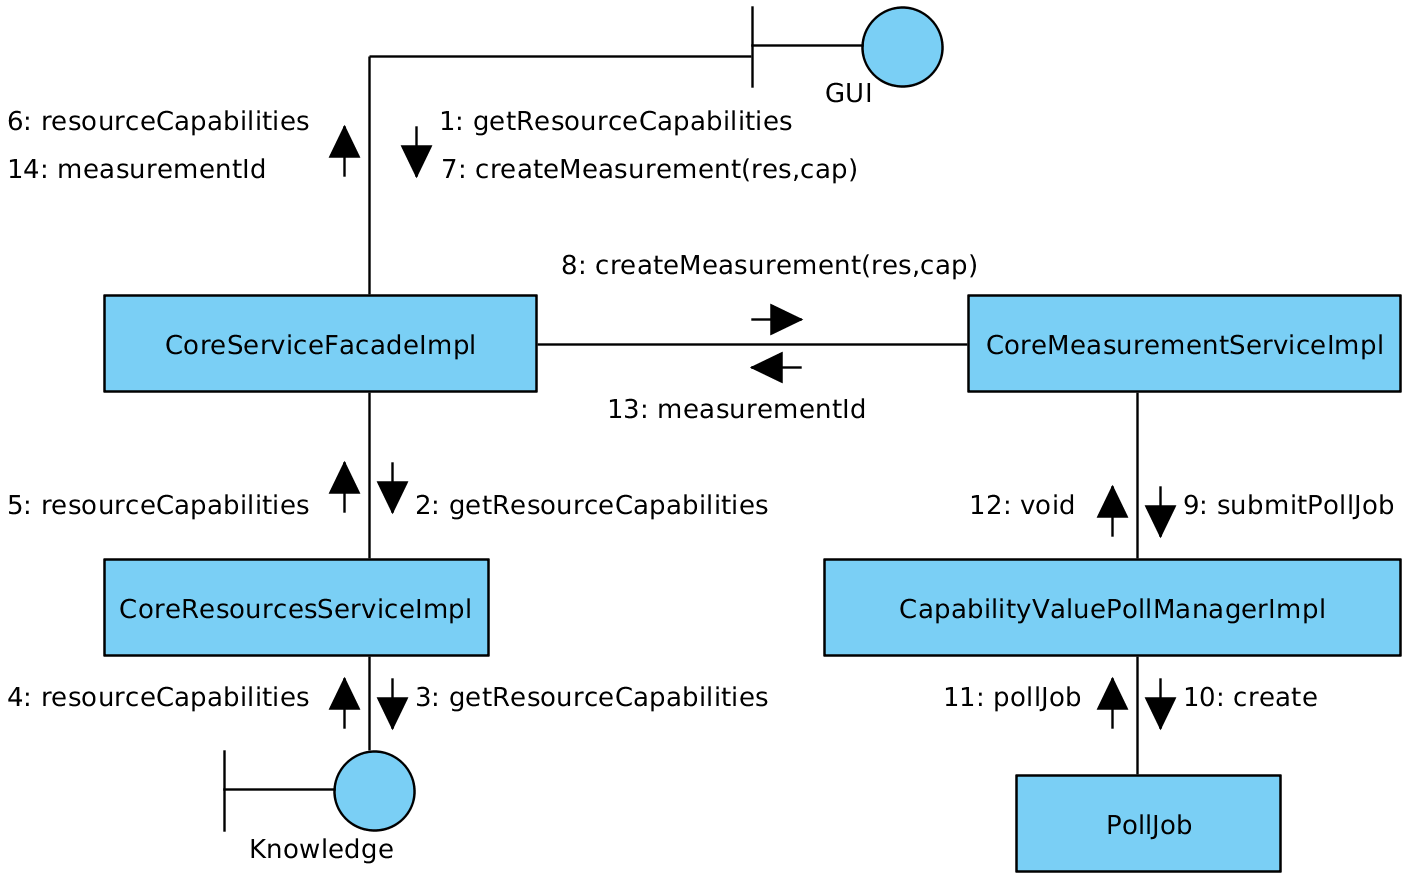
\includegraphics[width=0.8\textwidth]{comm_mh_add_measurement}
\caption{Monitoring Hub Communication diagram - adding new measurement}
\label{fig:comm_mh_add_measurement}
\end{figure}

Last data flow covered in this section describes gathering and publishing capability values. This time, CapabilityValuePollManagerImpl initiates the action. Its internal scheduler triggers previously created PollJob which contains measurement definition (URI's of resource and capability). Using those identifiers, PollJob calls CoreMeasurementServiceImpl to getCapabilityValue. Measurement service first looks up a transport proxy using TransportProxiesManagerImpl and then, using external TransportProxy, gets the capability value. In a subsequent step, gathered capability value is being pushed to all listeners, either directly (to listeners registered at CoreMeasurementServiceImpl) or using CoreRemoteServiceImpl to all remote listeners. What should be noticed here is that CoreRemoteServiceImpl notifies remote listeners in asynchronous and aggregated manner.

\begin{figure}[ht]
\centering
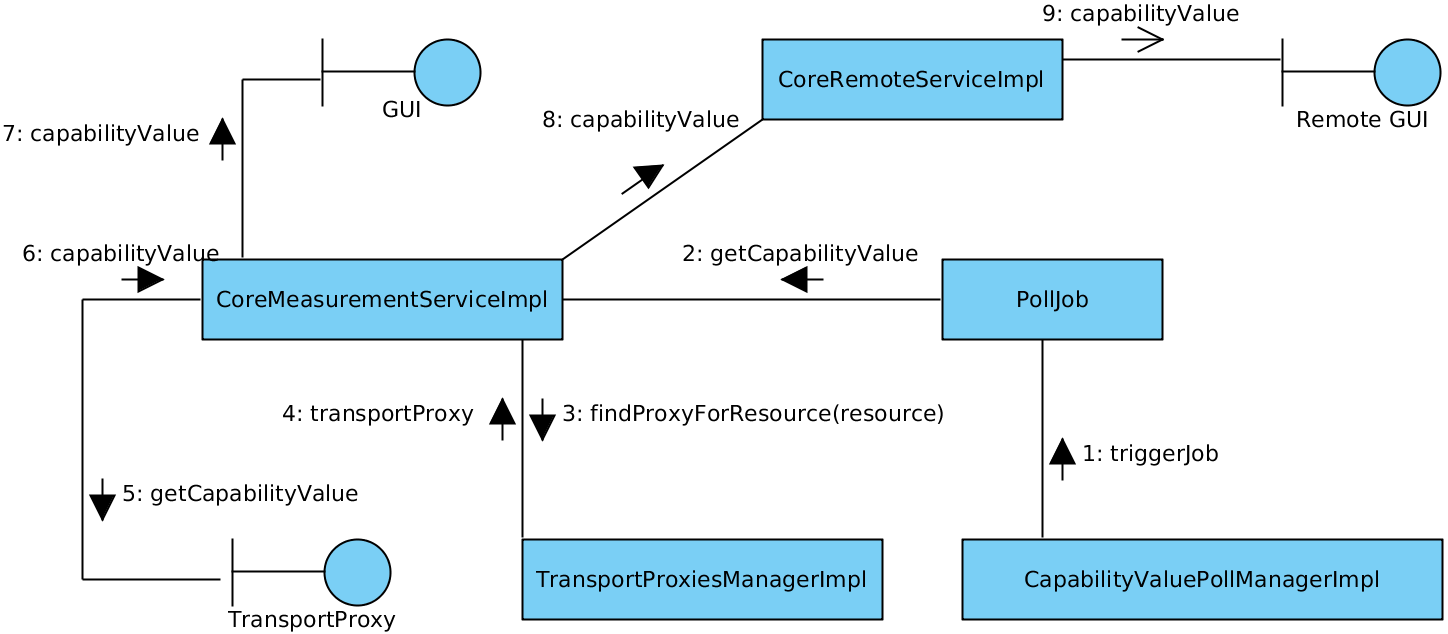
\includegraphics[width=1\textwidth]{comm_mh_new_cap_val}
\caption{Monitoring Hub Communication diagram - new capability value notification}
\label{fig:comm_new_cap_val}
\end{figure}
\pagebreak
